\documentclass{subfiles}

\begin{document}
    \subsection{States of matter}
        % Sis is se wörst aidea eva

        Matter in general is found in three states, named \emph{solid}, \emph{liquid} and \emph{gaseous}. We will focus on the latter two, as they are the most relevant for our experiment. First we discuss the so called \emph{ideal Gas} in the following section. 

        \subsubsection*{Ideal Gas}
            An ideal Gas is characterized by the properties of molecules having \emph{no volume} and \emph{no interaction} with each other. This means that the molecules are considered to be point-like. This assumption leads to the most fundamental equation in this experiment, the \emph{ideal gas law}:
            \[
                pV = nRT,
            \]
            where $p$ is the pressure, $V$ the volume, $n$ the number of moles, $R$ the universal gas constant and $T$ the temperature ´\footnote{The universal gas constant is given by $R = \SI{8.314}{\joule\per\mole\per\kelvin}$, found in \cite{nist:gasconstant}.} \cite[p.11]{nolting42}. 

        \subsubsection*{Real Gas}
            The introduced assumptions in ideal gas theory are in practice only met when infinitely decreasing density. \emph{Infinitely} in reality is not achievable, so the assumptions need a refresh. We assign every gasmolecule a volume $V_m$ and a force $F_m$ resulting interaction with close molecules. Doing this we enter the realm of \emph{real gas theory}, in which multiple models exist. One of them is the \emph{van der Waals} model, in which coefficients $a$ and $b$ are introduced to account for the volume and interaction of the molecules. The van der Waals equation is then given by
            \[\nbra{p + \frac{a\cdot n^2}{V^2}} \cdot \nbra{V - n\cdot b} = nRT.\]
            The coefficients $a$ and $b$ are specific to each type of gas. \cite[p.13]{nolting42}
    
    \subsection{Thermodynamic aspects}
        Some of the typical thermodynamic terms were already used above. We now want to introduce them in a more formal way.
        \subsubsection*{State variables}
            A so called \emph{state variable} in general is a variable that \emph{describes} the state of a system. In thermodynamics of gases, the most common state variables are \emph{pressure} $p$, \emph{volume} $V$, \emph{temperature} $T$ and \emph{number of moles} $n$ or \emph{total number of molecules} $N$ \cite[p.5]{nolting42}. While those are mostly self explanatory, the next state variables called \emph{inner energy} $U$ and \emph{entropy} $S$ needs some understanding. To do so, we need to introduce the concept of \emph{thermodynamic processes}.
        \subsubsection*{Thermodynamic processes}
            A thermodynamic process is a process in which a system changes its state variables. The first law of thermodynamics is an example of such. It states that the change of inner energy $dU$ from a state $x\in\Def{U}$ to a new state $x + h$ is equal to the \emph{heat} $dQ$ added to the system minus the \emph{work} $dW$ done by the system:
            \[dU(x)(h) = dQ(x)(h) + dW(x)(h),\quad h\in\Def{U}.\]
            We now found a description of $U$ using its derivative \cite[p.36]{nolting42}. For the entropy $S$ we use the introduced term \emph{heat} and its derivative: $dS(x)(h) = dQ(x)(h) / dT(x)(h)$ \cite[p.56]{nolting42}. This leads us to another important aspect of thermodynamics, the \emph{thermal capacity}.

        \subsubsection*{Thermal capacity}
            The thermal capacity $C_S$ is the derivative of the Function $Q$, the so named heat function of the system, which is dependent on the state variable vector $x\in\R^d$ \cite[p.37-38]{nolting42}. When we partially derive $Q$ with respect to one or multiple of the vector components, the leftover components are considered constant. This leads to the following definition:
            \[C_S:=dQ(x)((\mbbEins_{S^c}(i))_{i\in X}),\quad X:=\Def{x}.\]
            For this we define $s$ as the set of indices which should be considered constant. The indicator function $\mbbEins_{X\setminus S}$ then creates the matching derivative vector on $S^c:=X\setminus S$. 

        \subsubsection*{Isentropic exponent}
            In an \emph{adiabatic process} no heat is added to the system. This means that $dQ(x)(h) = 0$ for every state $x$ and change $h$. Using the first law of thermodynamics and assuming ideal gas we can write
            \[dT(x)(V) = -\frac{p}{C_V} = \frac{n\cdot R}{C_V}\cdot\frac{T}{V},\]
            where we first used $dU(x)(V) = 0$ and $p = nRT/V$ and introduced $C_V$ as the \emph{thermal capacity} at constant volume. Using $nR = C_p-C_V$ and introducing $C_p$ as the \emph{thermal capacity} at constant pressure we find
            \[dT(x)(V) = \frac{C_p-C_V}{C_V} \cdot\frac{T}{V}.\]
            Now we can define the \emph{isentropic exponent} $\kappa$ as $\kappa:=C_P/C_V$ and find the \emph{adiabatic equation}
            \[T\cdot V^{1-\kappa} = \textit{const}. \Longleftrightarrow p\cdot V^\kappa = \textit{const}.\]

        \subsubsection*{Poisson equations}
            The \emph{poisson equation} in general is a partial differential equation of the form
            \[-\lap u(t) = F(t,u(t))\]
            with some right side $F\in C^0(\R\times\R^d)$ and the sought function $u\in C^2(\R^d)$.
    
    \subsection{Experimental principle}
        \subsubsection*{Rüchhardt and Flammersfeld}
            To measure the isentropic exponent $\kappa$, Rüchhardt and Flammersfeld developed the setup illustrated in \ref{fig:RuchardtFlammersfeld}.

            \begin{figure}[H]
                \centering
                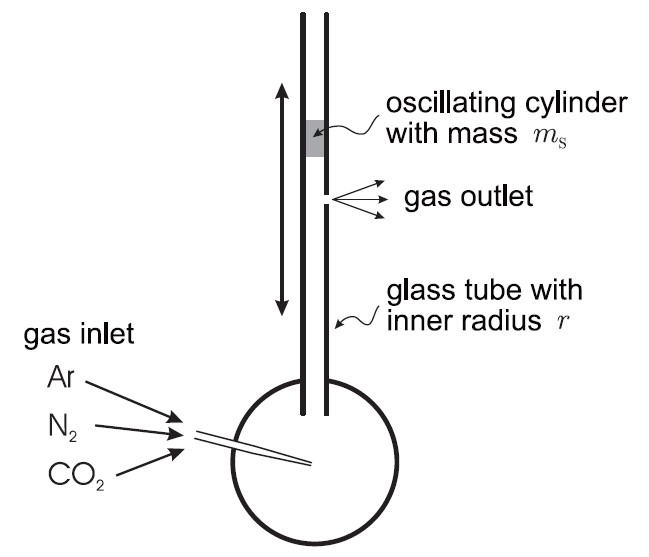
\includegraphics[width=6cm]{Bilddateien/Grundlagen/IsentropicRuchardtFlammersfeld.jpg}
                \caption{A cylinder $m_S$ oscillators due to gravitational forces, the air pressure $p_0$ and gas pressure of a gas $Ar$, $N_2$, $CO_2$ acting on it}
                \label{fig:RuchardtFlammersfeld}
            \end{figure}

            \noindent In equlibrium, the pressure of the gas is equal to $p_0$ plus the pressure caused by the gravitational force $F_G$:
            \begin{align*}
                p=p_0+\frac{F_G}{A}=p_0+\frac{m_S\cdot g}{\pi^2}.
            \end{align*}
            As no heat is transferred during the oscilating of the cylinder, we have $p\cdot V^{\kappa}=const.$ or $p\propto V^{-\kappa}$. Taking the Differential of this expression leads, after some more steps, to the equation 
            \begin{align*}
                m\cdot \ddot x(t)+\frac{\kappa\cdot p\cdot \pi^2\cdot r^4}{V}\cdot x(t)=0
            \end{align*} 
            with
            \begin{itemize}
                \item $m$: total mass of cylinder $m_S$ and gas
                \item $V$: volume of gass in equlibrium
                \item $r$: radius of cylinder/ gas tube
                \item $x$: spatial displacement of cylinder from state of equlibrium
            \end{itemize}
            This is the differential equation of the undamped harmonic oscillator, which yields the oscillation period $T=\sqrt{\frac{4\cdot m\cdot V}{\kappa\cdot p\cdot r^4}}$ ($p$: pressure in equlibrium). As $T$ is easily measurable, one can such computer the isentropic exponent \cite[p.259-262]{skript}
            \begin{align*}
                \kappa=\frac{4\cdot m\cdot V}{T^2\cdot p\cdot r^4}
            \end{align*}

        \subsubsection*{Clément and Desormes}
            An alternative measurement of $\kappa$, described by Clément and Desormes, is shown in figure \ref{fig:ClementDesormes}.
            
            \begin{figure}[H]
                \centering
                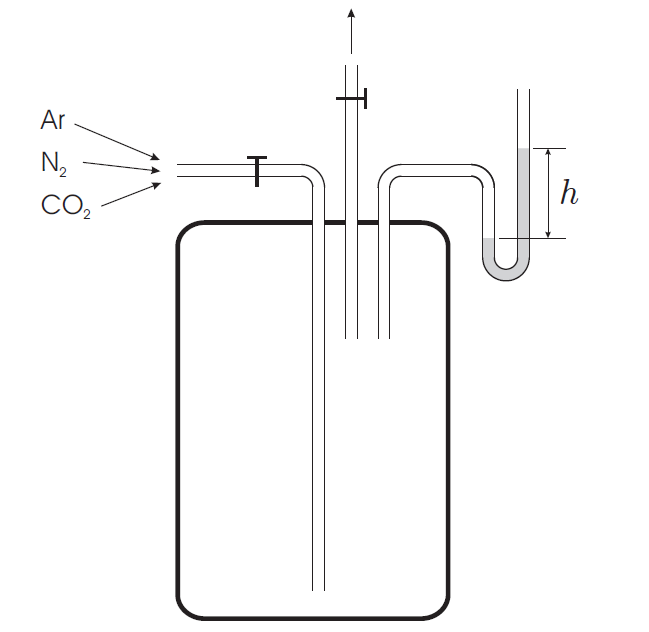
\includegraphics[width=6cm]{Bilddateien/Grundlagen/IsentropicClementDesormes.png}
                \caption{A cylinder $m_S$ oscillators due to gravitational forces, the air pressure $p_0$ and gas pressure of a gas $Ar$, $N_2$, $CO_2$ acting on it}
                \label{fig:ClementDesormes}
            \end{figure}

            The experiment is divided into two parts:
            \begin{itemize}
                \item A Gas is filled into the glass bottel in \ref{fig:ClementDesormes} such that the pressure $p_1$ inside the bottle is higher than the outside pressue $p_0$. The difference in pressure can now be calculated via the height of the water pillar in the small tube attached to the glass:
                \begin{align*}
                    p_1-p_0=\rho_{Water}\cdot g\cdot h_1
                \end{align*} 
                \item Some amount of gas is then let out through a valve such that the inner pressue $p_2$ is equal to $p_0$ (indicated by $h_2=0$): the Volume of the gas expands in an approximatially isentropic process and the temperature drops. When the valve is closed again, the gas heats up in an isochor process. The final pressure $p_3$ can once more be calculated using the height $h_3$ of the water pillar.\\
                
                \noindent Applying the poison equation to the isentropic, and the \textit{law of Charles} to the isochor process then yields
                \begin{align*}
                    p_3-p_0\approx(p_1-p_0)\cdot\frac{\kappa-1}{\kappa}
                \end{align*}
            \end{itemize}
            Finally, $\kappa$ is given as 
            \begin{align*}
                \kappa\approx\frac{p_1-p_0}{(p_1-p_0)-(p_3-p_0)}=\frac{h_1}{h_1-h_3}.
            \end{align*} 


% ideal gas
% state variables + thermodynamic processes
% 1. law of thermodynamics
% isentropic exponent + Poisson équations: show connections to degrees of (but no derivation of Poission equations required, good for us)
% thermal capacity
\end{document}